\chapter{反激式开关电源变换器工作机制}
本章研究开关电源的工作机制,首先阐述反激式开关电源的拓扑结构,然后分析反激式开关电源的各种工作模式、脉宽调制方式、不同的环路控制方式和两种反馈方式。为后续完成芯片工作流程与功能模块的构建,根据芯片应用电路和功 能对系统的外围器件和内部参数指标进行设计。

\section{拓扑结构分析}
反激式 AC/DC 变换器的主要功能为将从交流电整流得到的直流高压转化为目标 负载所需要的输出电压。主要适用于中小功率的应用场景,其本身由Buck-boost拓扑衍生而来,考虑到对电路安全性要求较高,在常规的 buck-boost结构中加入变压器取代电感线圈发展出电气隔离结构,即隔离型反激式变换器。

\subsection{传统反激式拓扑结构}

反激式变换器拓扑通过使用变压器代替Buck-boost电路中的单电感,不仅能够储能和能量传递,还能实现电气隔离的作用,将未稳定的原边电压和稳定的输出电压隔离开来。该拓扑的电气隔离有效地切断了变压器原副边之间无用信号的传递,不但防止了原边危险的瞬态高压耦合到副边,还断开了原副边的接地回路,提高了输出信号的抗噪声能力,可以实现相比于普通Buck-boost电路更大的功率优势。传统反激式开关电源变换器系统的拓扑结构如图~\ref{fig:传统反激式拓扑图}所示。

\begin{figure}[htbp] 
    \centering
    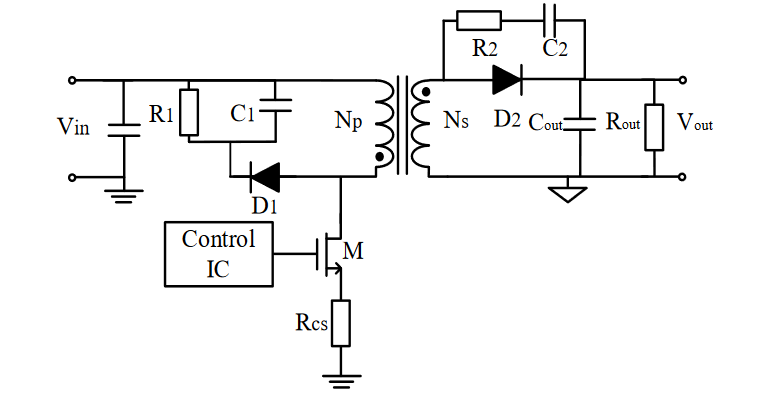
\includegraphics[width=0.6\linewidth]{figures/传统反激式拓扑图.png}
    \caption{传统反激式拓扑图}
    \label{fig:传统反激式拓扑图}
\end{figure}

该变换器系统的拓扑核心结构包括原副边极性相反的变压器、功率开关管、电流采样电阻、副边续流二极管、输出电容和输出负载电阻。功率管开关管的栅极连接变换器芯片的驱动信号,控制功率管的开启和关断;漏端连接在变压器的下边沿,源端连接采样原边电感电流的采样电阻。副边续流二极管的正端连接着变压器副线圈的上边沿,负端连接着输出电容和输出负载电阻。除了核心结构外,拓扑中还包括了RCD尖峰电流吸收电路和二极管保护电路等结构。由于实际的变压器中存在漏感,当功率管在硬开关的条件下被栅极驱动信号关断后,原边电感电流会产生的尖峰信号,加入由电阻、电容和二极管组成的吸收电路可以通过合理消耗漏感的能量来抑制尖峰电流信号的大小;同时考虑到安全性的问题,为了减小副边续流二极管的反向恢复应力,在续流二极管上并联电阻和电容元件,保护续流二极管不会在功率管导通和关断时被烧毁。


\subsection{非对称半桥反激式拓扑结构}

非对称半桥反激式(Asymmetric Half-Bridge Flyback)开关电源变换器拓扑是由传统反激式电路的副边结构和LLC电路的原边结构组合而成,后续简称为AHB反激式。该拓扑结构结合了反激式拓扑和LLC拓扑的优点,既可以利用变压器的漏感实现功率管在全工作范围下的软开关,极大地降低开关损耗,又能通过回收寄生元器件的能量进而提高转换效率,降低变压器的体积,是当前针对中等功率领域极有优势的拓扑结构。

\begin{figure}[htbp] 
    \centering
    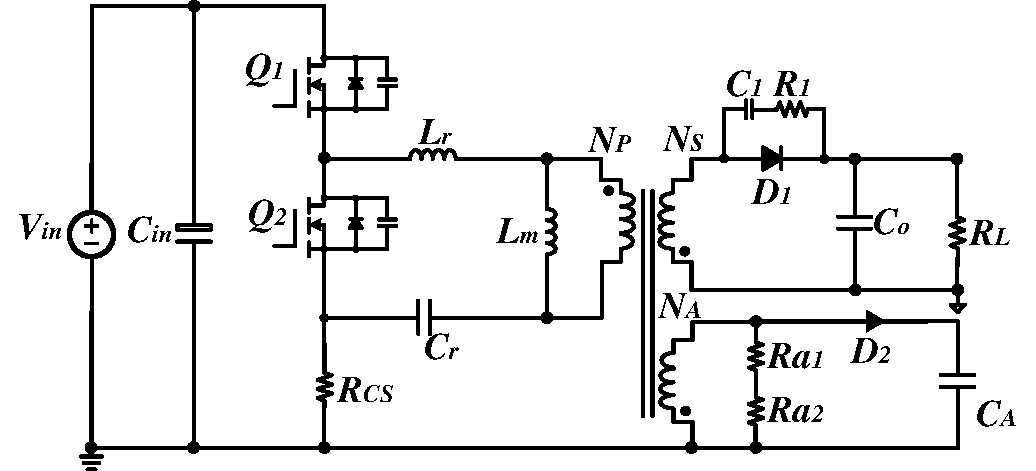
\includegraphics[width=0.8\linewidth]{figures/AHB拓扑图.pdf}
    \caption{AHB反激式拓扑图}
    \label{fig:AHB拓扑图}
\end{figure}

AHB反激式变换器拓扑结构电路如图~\ref{fig:AHB拓扑图}所示。该拓扑的原边电路包括两个功率管开关管$Q_1$和$Q_2$、采样电阻$R_{CS}$、变压器的原边励磁电感$L_m$和漏感$L_r$,以及与变压器和采样电阻串联的谐振电容$C_r$,原边电路类似于LLC变换器,$L_m$、$L_r$$C_r$共同组成串联谐振腔,显示了AHB反激式变换器电路的谐振特性,回收变压器的漏感能量,进而降低变压器体积和提高效率;变压器的副边电路和传统反激式变换器结构的副边相似,由续流二极管$D_1$、输出电容$C_o$和输出负载电阻$R_L$组成,续流二极管两端同样并联电阻$R_1$和电容$C_1$抑制续流二极管的反向恢复应力,此种电路结构可以为变换器系统提供较宽的输出范围。

特别的是该拓扑还包括一个辅助绕组,包括分压电阻$R_{a1}$和$R_{a2}$、续流二极管$D_1$和供电电容$N_A$。该辅助绕组不仅可以通过二极管和电容为变换器芯片提供稳定的供电电压,还可以通过电阻$R_{a1}$和$R_{a2}$分压后为变换器提供额外的电路信息,如检测输出电压的大小和检测副边电流的零电流导通时刻(ZCS),确保功率管在全工作模式下都实现零电压导通(ZVS)的软开关,从而实现更高的能量转换效率。




\section{工作原理}

非对称半桥反激式开关电源变换器的简化拓扑结构如图~\ref{fig:AHB简化拓扑图}所示。该图中$V_{in}$为直流输入电压;变换器系统中的高低边功率管$Q_1$和$Q_2$的栅极驱动信号分别为占空比为D的HSGD和占空比为1-D的LSGD。每个功率管都包含一个体二极管和寄生电容。谐振电容$C_r$在低边功率管$Q_2$导通时近似为一个恒定的直流源;变压器原边线圈匝数为$N_P$,副边线圈匝数为$N_S$,原边和副边的匝数比为N。输出端D为副边续流二极管,$C_o$为输出滤波电容,R为输出负载电阻。

\begin{figure}[htbp] 
    \centering
    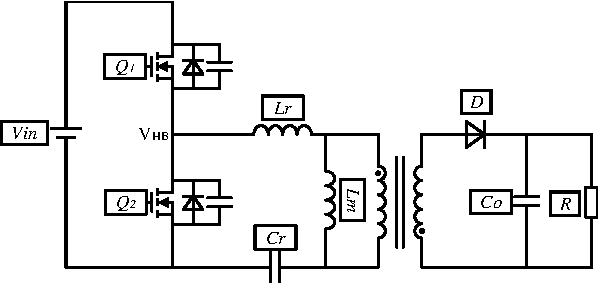
\includegraphics[width=0.6\linewidth]{figures/AHB简化拓扑图.pdf}
    \caption{AHB简化拓扑图}
    \label{fig:AHB简化拓扑图}
\end{figure}

\begin{figure}[htbp] 
    \centering
    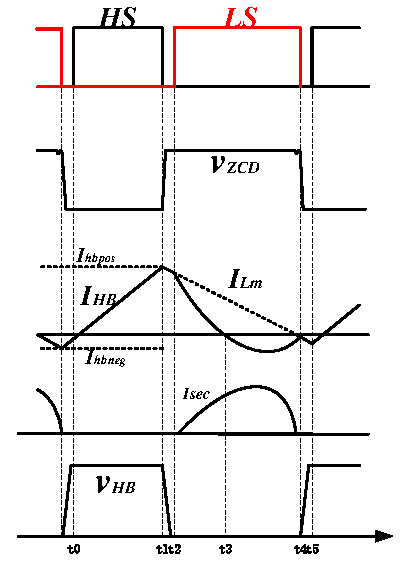
\includegraphics[width=0.6\linewidth]{figures/BCM工作波形图.pdf}
    \caption{AHBF BCM工作波形图}
    \label{fig:BCM工作波形图}
\end{figure}
								
非对称半桥反激变换器工作在临界导通模式时的主要工作波形如图~\ref{fig:BCM工作波形图}所示。图中从上到下分别是高低边功率管$Q_1$和$Q_2$的电压驱动波形HS和LS、辅助绕组电压分压ZCD引脚电压$V_{ZCD}$的波形、变压器原边励磁电感电流$I_{LM}$和原边电感电流$I_{HB}$的波形、变压器副边电感电流$I_{sec}$的波形,高低边功率管半桥节点电压$V_{HB}$的波形。该控制模式下共分为5个阶段。
						


\begin{figure}[htbp] 
    \centering
    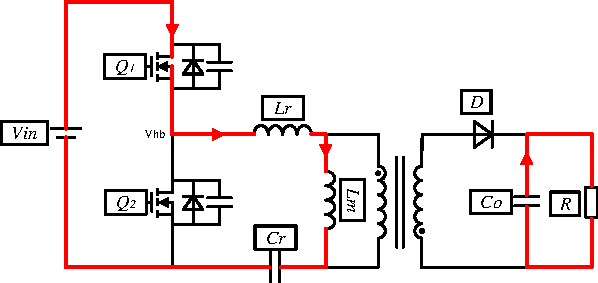
\includegraphics[width=0.6\linewidth]{figures/工作原理1.pdf}
    \caption{阶段1 ($t_0 \thicksim t_1$)}
    \label{fig:工作原理1}
\end{figure}
                
阶段1,$t_0 \thicksim t_1$:此阶段在$t_0$时刻高边功率管$Q_1$完全导通,低边功率管$Q_2$保持关断状态,如图~\ref{fig:工作原理1}所示。半桥节点电压$V_{HB}$等于输入电压$V_{in}$,原边电感电流$I_{HB}$正向流动,输入电压$V_{in}$对原边励磁电感$L_m$、变压器漏感$L_r$和谐振电容$C_r$进行充电,此时原边励磁电感$L_m$、变压器漏感$L_r$和谐振电容$C_r$共同构成谐振回路,由于谐振周期很大,远远大于一个开关周期,其谐振作用在一个开关周期中并不十分明显,因而电感电流近似线性增加。谐振电容$C_r$上的能量持续增加,变压器原边电感电压上正下负,由于变压器的反向作用,副边电感电压上负下正,副边二极管D反向偏置,阻止副边电流$I_{sec}$的产生,输出负载由输出电容提供能量。

在该阶段内,根据回路电压为零和节点电流为零公式,可建立如下方程:
\begin{equation}
    \label{eq:回路电压公式}
    (L_m + L_r)\frac{di_r}{dt} = V_{in} - V_{Cr}  
\end{equation}
\begin{equation}
    \label{eq:结点电流公式}
    V_{Cr}\frac{dV_{Cr}}{dt} = i_r 
\end{equation}

由式\eqref{eq:回路电压公式}和\eqref{eq:结点电流公式}可计算得下式:
\begin{equation}
    \label{eq:Ihb公式1}
    i_{hb}(t) = i_{Lm}(t) = \frac{V_{a}-V_{Cr}(t)}{Z_o}\sin[\omega_o(t-t_0)] + I_{hbneg}\cos[\omega_o(t-t_0)]  
\end{equation}
\begin{equation}
    \label{eq:Vcr_2}
    V_{Cr}(t) =V_{a}-[V_{a}-V_{Cr}(t_0)]\cos[\omega_o(t-t_0)] + {Z_o} I_{hbneg} \sin[\omega_o(t-t_0)]
\end{equation}
其中,特征阻抗值的公式为:
\begin{equation}
    \label{eq:Zo公式}
    Z_o=\sqrt{\frac{L_m+L_r}{C_r}}  
\end{equation}
谐振角频率的公式为:
\begin{equation}
    \label{eq:omega_o公式}
    \omega_o=\frac{1}{\sqrt{C_r(L_m+L_r)}}
\end{equation}
$V_{a}$的公式为:
\begin{equation}
    \label{eq:Vhb公式1}
    V_{a}=V_{in}
\end{equation}

由于谐振角频率$\omega_o$很大,原边电感电流和励磁电流可近似表示为式\eqref{eq:Ihb公式2}:
\begin{equation}
    \label{eq:Ihb公式2}
    i_{hb}(t) = i_{Lm}(t) = I_{hbneg} + \frac{V_{in}-V_{Cr}(t)}{L_m + L_r}(t-t_0)
\end{equation}


\begin{figure}[htbp] 
    \centering
    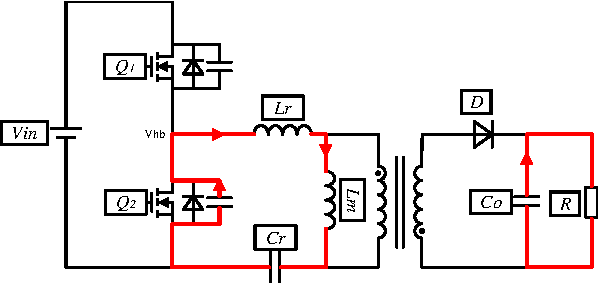
\includegraphics[width=0.6\linewidth]{figures/工作原理2.pdf}
    \caption{阶段2 ($t_1 \thicksim t_2$)}
    \label{fig:工作原理2}
\end{figure}
                
阶段2,$t_1 \thicksim t_2$:此阶段在$t_1$时刻关断高边功率管$Q_1$,同时低边功率管$Q_2$仍保持关断状态,如~\ref{fig:工作原理1}所示,进入功率管死区时间,断开充电路径与 $V_{in}$ 的连接。由于电感电流不能突变,原边电感电流持续正向流动并逐渐减小,对低边功率管$Q_2$的寄生电容进行放电,迫使半桥节点电压$V_{HB}$下降,直到$t_2$时刻低边功率管$Q_2$的体二极管开始导通,$V_{HB}$电压近似为0,为低边功率管的ZVS导通提供准备,此时变压器原边电感两端压降与电容器$C_r$的电压保持一致。输出负载仍由输出电容提供能量。此阶段由于副边二极管仍未被正向偏置,谐振回路未发生变化,特征阻抗值和谐振频率未变仍如式\eqref{eq:Zo公式}和式\eqref{eq:omega_o公式},故原边电感电流和励磁电流仍然相等,但由于$V_{HB}$的近似为0,重新带入式\eqref{eq:Ihb公式1}和式\eqref{eq:Vcr公式}中可将原边电感电流和励磁电感电流公式可近似为式\eqref{eq:Ihb公式3}:
\begin{equation}
    \label{eq:Ihb公式3}
    i_{hb}(t) = i_{Lm}(t) = I_{hbpos} - \frac{N_P}{N_S} \frac{V_o}{L_m + L_r}(t-t_1)
\end{equation}

                
\begin{figure}[htbp] 
    \centering
    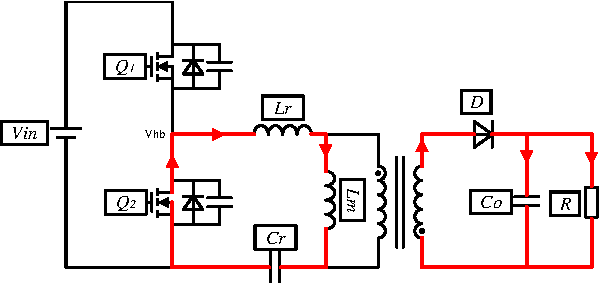
\includegraphics[width=0.6\linewidth]{figures/工作原理3.pdf}
    \caption{阶段3 ($t_2 \thicksim t_3$)}
    \label{fig:工作原理3}
\end{figure}

阶段3,$t_2 \thicksim t_3$:此阶段在t2时刻低边功率管$Q_2$在栅极信号的驱动下顺利在ZVS条件下实现导通,极大地降低了开关损耗,高边功率管$Q_1$仍保持关断状态,如~\ref{fig:工作原理3}所示。功率管中间半桥节点电压$V_{HB}$为零,变压器原边电感极性发生变化,电感电压变为上负下正,经变压器反向后副边电感电压上正下负,副边电感电压等于谐振电容两端电压$V_{Cr}$除以变压器匝数比N,副边二极管D正向偏置自然导通,同时原边励磁电感被输出电压箝位,励磁电感电压的公式为:$V_{Lm}=NV_o$,$L_m$不再参与谐振,谐振电容$C_r$只与变压器的漏感$L_r$发生串联谐振,由于变压器漏感$L_r$和谐振电容$C_r$的谐振周期较小,小于开关周期,可见图中初级侧电感电流呈谐振式持续减小直至正向电流为零。存储在励磁电感中的电能开始通过变压器向副边转移,副边电感电流$I_{sec}$开始逐渐增大。因为副边电流的存在,原边电感电流和励磁电流不再相等,原边电感电流和励磁电感电流的公式分别可表示为式\eqref{eq:Ihb公式4}和\eqref{eq:Ihb公式5}:
\begin{equation}
    \label{eq:Ihb公式4}
    i_{hb}(t) = \frac{\frac{N_P}{N_S}V_o - V_{Cr}(t)}{Z_r}\sin[\omega_o(t-t_2)] + i_{hb}(t_2) \cos[\omega_o(t-t_2)]  
\end{equation}
\begin{equation}
    \label{eq:Ihb公式5}
    i_{Lm}(t) = i_{hb}(t_2) - \frac{N_P}{N_S} \frac{V_o}{L_m}(t-t_2)
\end{equation}
其中,特征阻抗值的公式为:
\begin{equation}
    \label{eq:Zr公式}
    Z_r=\sqrt{\frac{L_r}{C_r}}  
\end{equation}
谐振角频率的公式为:
\begin{equation}
    \label{eq:omega_r公式}
    \omega_r=\frac{1}{\sqrt{C_r L_r}}
\end{equation}
由于励磁电感电流等于原边电感电流和经变压器反射后的副边电流之和,如式\eqref{eq:Ihb公式6}所示,将式\eqref{eq:Ihb公式4}和\eqref{eq:Ihb公式5}带入其中可求得副边电流公式\eqref{eq:Isec公式1}:
\begin{equation}
    \label{eq:Ihb公式6}
    I_{Lm} = I_{HB} + \frac{N_P}{N_S}I_{sec}
\end{equation}
\begin{equation}
    \label{eq:Isec公式1}
    i_{sec}(t) 
    %&= \frac{N_P}{N_S}[i_{Lm}(t) - i_{hb}(t)] \\ &
    = \frac{N_P}{N_S} i_{hb}(t_2) \{  1 - \cos[\omega_r(t-t_2)]\}  - \frac{N_P^2}{N_N^2} \frac{V_o}{L_m} (t-t_2)
    - \frac{\frac{N_P^2}{N_S^2} V_o - V_{Cr}}{Z_r} \sin[\omega_r(t-t_2)]
\end{equation}
随着副边电流的逐渐增大,原边电感电流在$t_3$时刻正向降低为零,该阶段结束。



\begin{figure}[htbp] 
    \centering
    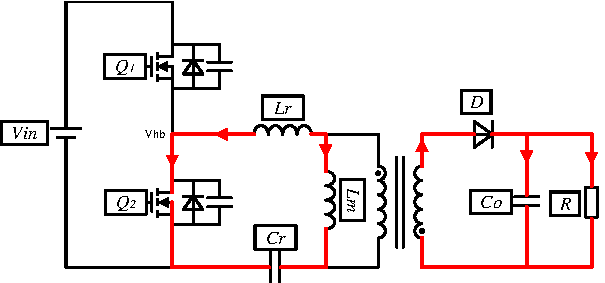
\includegraphics[width=0.6\linewidth]{figures/工作原理4.pdf}
    \caption{阶段4 ($t_3 \thicksim t_4$)}
    \label{fig:工作原理4}
\end{figure}

阶段4,$t_3 \thicksim t_4$:此阶段高低边功率管$Q_1$和$Q_2$仍保持上一阶段状态,在$t_3$时刻原边电感电流正向降低为零,开始负向流动并持续增大,如~\ref{fig:工作原理4}所示。此时谐振电容$C_r$和励磁电感$L_m$共同为副边提供能量。同时,励磁电感电流也逐渐降低至与原边电感电流相等的值,如~\ref{fig:BCM工作波形图}中$t_4$时刻所示,此时励磁电感能量全部退磁完成,不再为副边提供能量,副边电感电流$I_{sec}$降低为零,辅助绕组电感电压分压$V_{ZCD}$波形上出现高频谐振,这是因为副边二极管寄生电容和变压器漏感发生的谐振现象,这一反映励磁电感退磁完成的高频谐振波形可以作为判断低边功率管关断的关键信号,故在$t_4$时刻低边功率管在栅极信号驱动下开始关断。

\begin{figure}[htbp] 
    \centering
    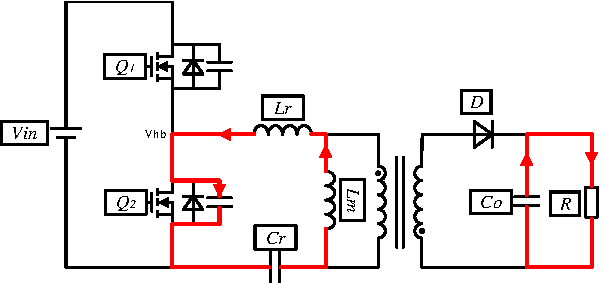
\includegraphics[width=0.6\linewidth]{figures/工作原理5.pdf}
    \caption{阶段5 ($t_3 \thicksim t_4$)}
    \label{fig:工作原理5}
\end{figure}
                
阶段5,$t_4 \thicksim t_5$:此阶段高低边功率管都保持关断状态,再次进入功率管的死区时间,如~\ref{fig:工作原理5}所示。由于励磁电感内存储的能量已全部传递到变压器副边,副边二极管在ZCS条件下自然关断,输出电压不再箝位励磁电感,励磁电感和变压器漏感共同和谐振电容串联谐振,特征阻抗值恢复为$Z_o$,谐振角频率恢复为$\omega_o$,谐振周期远远大于开关周期,原边电感电流和励磁电感电流如\eqref{eq:Ihb公式2}所示,因为电感电流无法进行突变,电感电流仍负向流动,对低边功率管$Q_2$寄生电容进行充能,逐渐拉高半桥节点电压$V_{HB}$,直至$t_5$时刻半桥节点电压$V_{HB}$被高边功率管$Q_1$中的体二极管钳位,$V_{HB}$近似等于输入电压,电路达到开启高边功率管$Q_1$的ZVS条件,至此,一个周期结束。

								
%阶段1,$t_0$-$t_1$:此阶段在$t_0$时刻高边功率管$Q_1$完全导通,低边功率管$Q_2$保持关断状态,进入功率%管死区时间。



\section{开关电源的工作模式}
\label{sec:dataset-build}
\subsection{CCM连续导通模式}
对于非对称半桥反激式开关电源变换器而言,不同于传统的反激式开关电源变换器,连续导通模式是指,当系统给出功率开关管的下一周期导通信号时,变压器原边电感电流和励磁电感电流未重合,变压器励磁电感中的能量还没有完全退磁转移到次级侧负载,紧接着又从输入端开始继续获取能量。

非对称半桥反激式开关电源变换器在连续导通模式下的波形如下图所示,tHSon是高边功率管HS的导通时间,tLSon是低边功率管LS的导通时间,$V_{HB}$是高低边功率管的中间节点电压,VCr是初级侧谐振电容的两端电压差,Ihb是初级侧电感电流,ILm是励磁电感电流,Isec是次级侧电感电流。

当高边功率管导通时,输入电压的能量在变压器励磁电感和谐振电容中积累,当高边功率管关断时,励磁电感和谐振电容中的能量经由副边绕组传递到输出端。当下一周期高边功率管导通再次开始励磁时,变压器励磁电感和谐振电容中储存的能量还未完全退磁传递到副边绕组的工作模式就是CCM模式。

在输入输出电压稳定运行期间,对励磁电感应用伏秒平衡原理,能够得到输入电压、输出电压和占空比D之间的关系。在tHSon内,励磁电感两端电压为输入电压减去谐振电容电压Vcr;在tLSon内,励磁电感两端电压为谐振电容电压Vcr,由此可得式\eqref{eq:CCM_1}:
\begin{equation}
    \label{eq:CCM_1}
    D\times(V_{in}−V_{cr\_avg})=(1−D)\times V_{cr\_avg}
\end{equation}
\begin{equation}
    \label{eq:Vcr_1}
    V_{cr\_avg}=N \times V_o\times\frac{L_m}{L_m+L_r}
\end{equation}
其中$V_{cr\_avg}$是谐振电容Cr上的平均电压,它等于输出电压经变压器原边励磁电感和漏感分压后乘以匝数比N。

对式\eqref{eq:CCM_1}和\eqref{eq:Vcr_1}进行整理可得式\eqref{eq:CCM_3}:
\begin{equation}
    \label{eq:CCM_3}
    V_o=D \times \frac{V_{in}}{N} \times\frac{L_m}{L_m+L_r}  
\end{equation}

根据式\eqref{eq:CCM_3}可知输出电压由占空比D、输入电压、变压器匝数比N、变压器励磁电感和漏感决定,与负载恒和频率无关。由于Lr对Lm而言非常小可以忽略不计,式\eqref{eq:CCM_3}可化简为式\eqref{eq:CCM_4}:
\begin{equation}
    \label{eq:CCM_4}
    V_o=D \times \frac{V_{in}}{N}  
\end{equation}

\subsection{DCM断续导通模式}




\subsection{CRM临界导通模式}




\section{开关电源的脉宽调制方式}
开关电源通过调节开关管控制信号的导通关断时间来改变信号占空比由此达到稳定输出电压或输出电流的目的,根据改变占空比方式的不同将会得到不同的开关电源调制方式,本节将分别介绍脉冲宽度调制(PWM)、脉冲频率调制(PFM)、脉冲跳周期调制(PSM)以及脉冲宽度频率调制(PWM-PFM)。

\subsection{PWM调制方式}
PWM调制的原理是指在功率管开关频率不变的情况下通过控制功率管管的导通时间来改变占空比的大小进而维持输出电压或输出电流的稳定,即定频调宽。这是开关电源变换器中最常用的一种调制方式,常见的PWM脉宽调制系统如下图所示,是将输出电压通过电阻串进行分压后产生的输出反馈信号Vfb与参考电压在误差放大器中进行比较,产生误差放大信号Vea,Vea再与频率固定的三角波信号在PWM比较器中比较,生产占空比不同的PWM控制信号来控制功率管的导通和关断,其中电压模的锯齿波信号由固定电路给定,电流模的锯齿波信号由原边电流采样电阻上的电压处理得到。

\begin{figure}[htbp] 
    \centering
    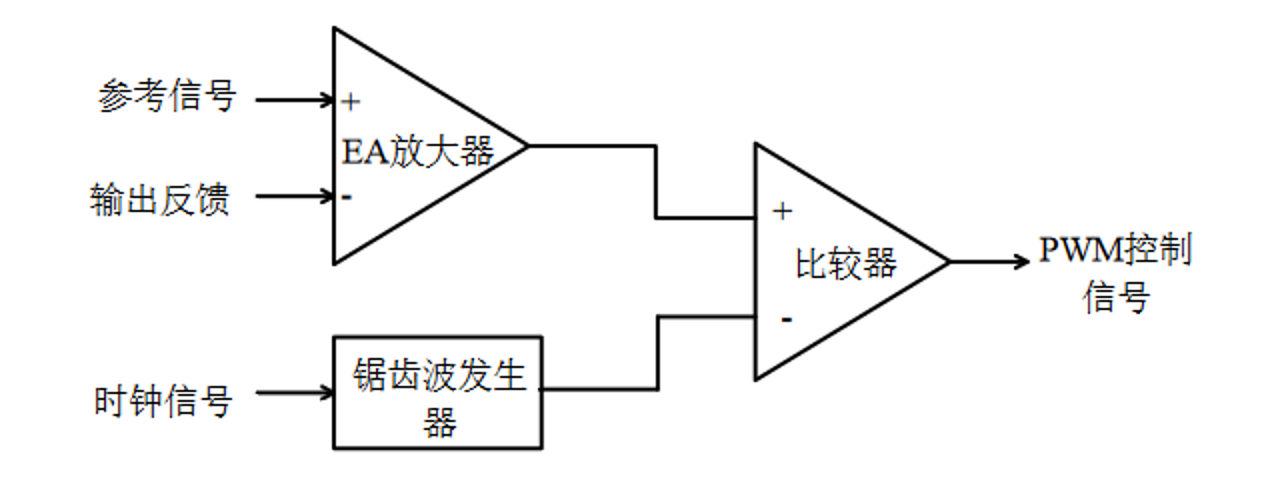
\includegraphics[width=0.8\linewidth]{figures/PWM调制1.png}
    \caption{PWM调制原理图}
    \label{fig:PWM调制1}
\end{figure}

当输出负载电流变大,输出负载会从输出电容中抽取能量,输出电压Vo变小,相应Vfb也变小,因此误差放大信号Vea增大,Vea与锯齿波信号比较后得到的脉冲宽度就会增大,导致PWM控制信号的占空比增大,将更多的能量在下一个周期中传递到副边电路维持输出电压的稳定。PWM调制作为最常用的调制方式,具有控制结构简单易于设计和实现、输出电压纹波小,动态响应快,线性度高,频率特性好等优点。但PWM调制由于频率固定,其更适用于重载情况下,因为不论输出负载大小如何,每个周期功率管都会进行导通关断操作,导致当输出负载处于空载和轻载情况下造成更多的开关损耗,电路的能量转换效率很低。

\subsection{PFM调制方式}
PFM调制的原理是指在功率管导通时间不变的情况下通过控制功率管的开关频率来改变占空比的大小进而维持输出电压或输出电流的稳定,即定宽调频。

常见的PWM脉宽调制系统如下图所示,同样是将输出电压通过电阻串进行分压后产生的输出反馈信号Vfb与参考电压在误差放大器中进行比较,产生误差放大信号Vea,不同于PWM调制,PFM调制的Vea信号输入到脉冲调制器中产生时钟信号CLK控制功率管的导通;功率管导通时长由原边电流采样电阻上的电压Vcs与给定的参考电压Vcsref比较所得的关闭信号控制。当脉冲调制器中
\subsection{PSM调制方式}
利用恒频恒宽进行调节的方式称为脉冲跳周期调制,这样一种全新的控制模式被 应用于开关功率变换器,当使用 PSM 调制时脉冲的宽度和频率保持恒定,这些脉冲 作为开关管的输入信号,所需要周期的个数会由负载的大小来进行决定。当参考电压 大于输出电压,恒定频率和宽度的时钟控制信号允许功率开关管在该周期中工作,当参考电压小于输出电压时,该周期将会被开关管忽略。PSM 调制模式其效率并不取决于输出功率,当负载发生变化时效率仍然保持恒 定,脉冲跳周期调制模式的优点是轻负载时的转换效率比脉冲宽度调制模式高、抗干扰能力强、静态功耗低;跳过一些工作周期后,会带来很大的输出电压波纹、线性调 整率变差、系统的有效频率降低等缺点。
\subsection{PWM+PFM调制方式}
PWM-PFM 是一种将 PWM 调制方法与 PFM 调制方法相结合的混合调制方法。 由上文分析可知,在高负载的情况下,PWM 调制方式效率更高,输出纹波小,开关频率固定,开关周期固定,因此针对 PWM 模式的噪声滤波器设计比较简单;但在负载较轻的情况下效率会降低,而 PFM 调制方法在轻载下频率会降低因而会有更高的 效率。PWM-PFM 混合调制方法具备 PWM 调制方法和 PFM 调制方法共同的优点。 PWM-PFM 混合调制模式兼具两种调制模式的优点,它既可以改变开关管控制信号的 频率,又可以改变控制信号脉冲宽度。在不同的负载情况下采用不同的方法使开关电 源的效率始终高于不考虑负载变化的情况,但混合调制方法对应的电路设计非常复杂,不同的控制回路需要设计采用不同的补偿结构。

\section{开关电源的环路控制方式}
为了使电路的输出端可以连接不同大小的负载,需要在输出电路中加入反馈电路 使输出达到稳定的状态,从而整个系统也能够继续稳定地工作。反馈环路是指输出端 采样到运放的输出端,被控对象是指运放输出到系统输出,在开关电源的设计中,反馈电路的性能会对开关电源的精度和总体性能产生巨大影响。因此,良好反馈回路的设计是开关电源系统开发的关键,开关电源既可以用电压也可以用电流控制,下 面对这两种模式的工作原理进行详细分析。

\subsection{电压控制模式}
电压控制环路属于单环路控制方式,只包含一个和输出电压信号相关的电压反馈回路,具有结构简单、设计容易和抗干扰能力强等优点。电压控制模式的典型电路如~\ref{fig:电压工作模式电路图} 所示,主要由误差放大器、振荡器、比较器、SR锁存器和驱动电路等组成。误差放大器的负输入端是辅助绕组采样输出电压后通过分压电阻串 R1、R2 得到的分压电压,正输入端是参考电压Vref,误差放大器通过放大分压电压和参考电压的差异生成误差放大信号VEA。当输出负载变化时会导致输出电压上冲或下冲,该变化会引起VEA的上下波动,因此VEA可以反映输出负载的变化,锯齿波信号与VEA通过比较器比较后即可在不同输出负载的情况下调节SR锁存器的复位时间,进而改变驱动模块生成的脉冲宽度大小。当负载电流减小,分压电压大于参考电压,误差电压信号VEA降低,从而VEA通过比较器和锯齿波电压信号比较后生成的输出信号更早得控制SR锁存器复位,驱动模块产生的控制高边功率管导通信号的脉宽变窄,降低对变压器副边的能量传递,将输出电压逐渐降低到标准范围,维持输出电压的稳定。

\begin{figure}[htbp] 
    \centering
    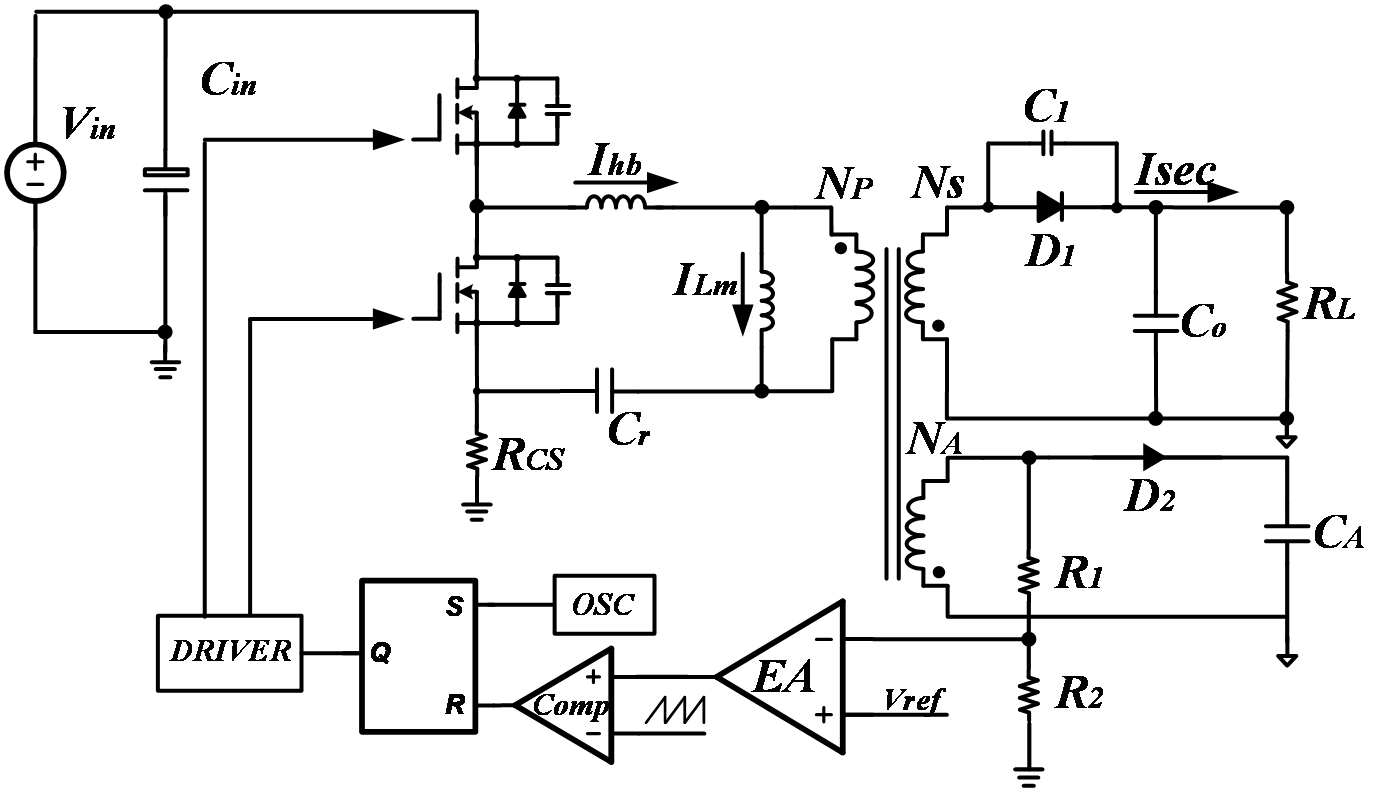
\includegraphics[width=0.8\linewidth]{figures/电压工作模式电路图.png}
    \caption{电压工作模式电路图}
    \label{fig:电压工作模式电路图}
\end{figure}

电压控制环路虽然结构简单且易于控制,但是由于只有一个电压环路,故只有当输出电压发生变化之后才会影响功率管的导通和关断时间,开始进行闭环负反馈动态调节,当输入电压产生干扰时,原边电感电流的上升斜率发生变化,会影响原边励磁电感的储能,但电压环路的控制和调节不会立即发生作用,而是在延迟一段时间之后才会起作用,系统整体的动态响应就会变差,输出电压产生很大的上冲和下冲现象。

\subsection{电流控制模式}

电流控制环路属于多环路控制方式,典型电路图如~\ref{fig:电流工作模式电路图}所示,包含一个电压环路和一个电流环路,电压环路和电压控制环路相同,采样输出电压信号用于生成误差放大信号;电流环路则是实时采样功率管的电流作为反馈电流,用采样电阻将电流转换为采样电压替代电压控制模式中的锯齿波信号,同误差放大信号VEA进行比较。

\begin{figure}[htbp] 
    \centering
    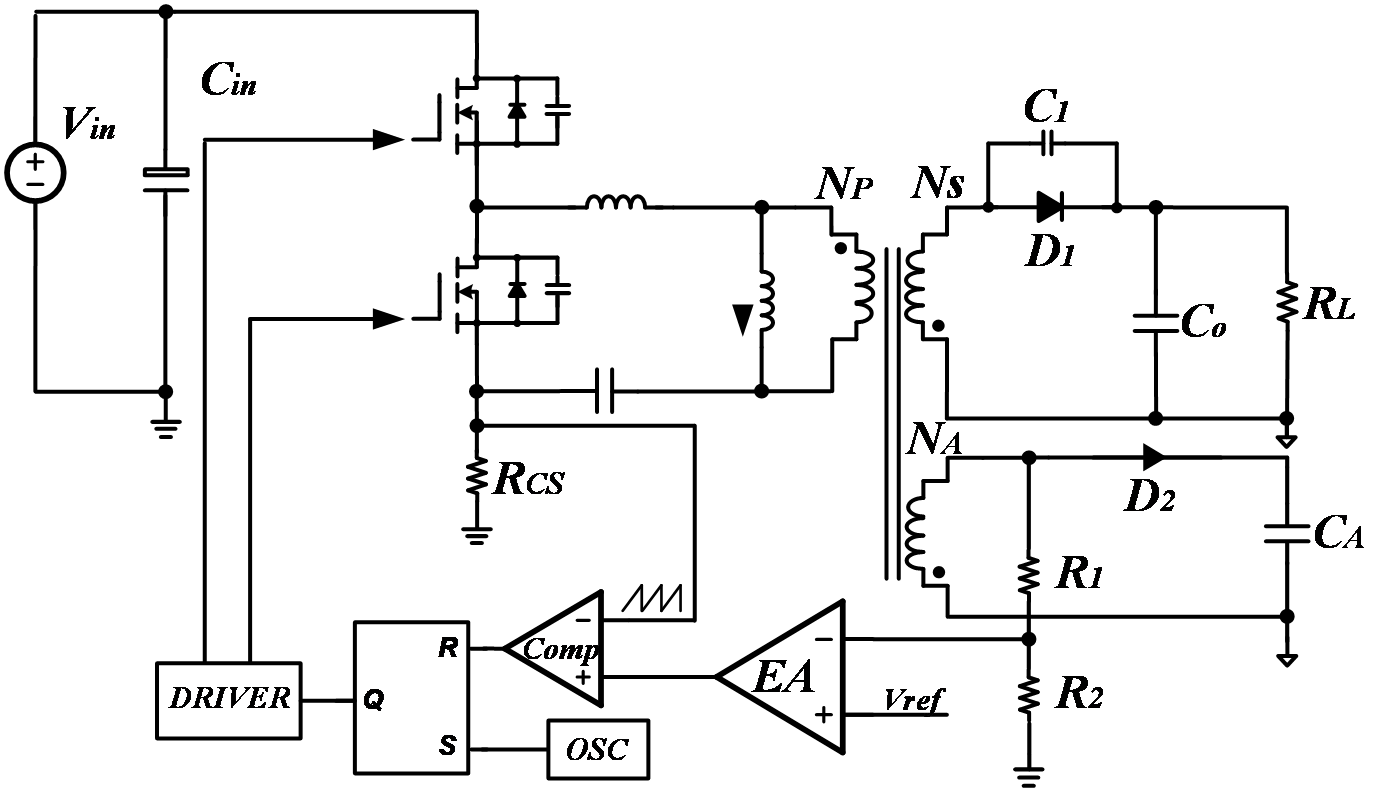
\includegraphics[width=0.8\linewidth]{figures/电流工作模式电路图.png}
    \caption{电流工作模式电路图}
    \label{fig:电流工作模式电路图}
\end{figure}

相比于电压控制模式对输入电压信号的不敏感,电流控制模式对输入输出信号都可以进行反馈,输入电压信号的变化会影响功率管导通时刻的电流斜率,通过采样电阻后产生一个随输入电压变化而变化的锯齿波信号,当输入电压发生扰动时,反馈环路可以直接响应改变功率管导通时间,而不需要等待输出电压信号发生相应波动后改变VEA的大小再影响功率管导通时间,极大地提高了系统整体的动态响应时间。但由于电流控制模式包含两个反馈环路,增大了电路结构的设计复杂度,另外,当驱动信号的占空比大于 50\%时,电路中不可避免地会出现次谐波振荡, 这需要增加额外的斜坡补偿电路来解决,一定程度上,也增加了应用难度。

 
\section{开关电源的反馈方式}
反激式开关电源变换器电路为保证输出电压稳定,进行闭环回路控制,需要对输出电压信号进行采样,并通过不同的方式将其反馈到变换器芯片进行逻辑处理。反激式开关电源变换器根据反馈结构的不同分为原边反馈(PSR)和副边反馈(SSR)两种反馈方式。其中原边反馈是通过辅助绕组对副边输出电压信号进行检测采样,副边反馈是通过 TL431 稳压模块和光耦模块组成的反馈系统对输出电压信号进行检测采样。

\subsection{原边反馈电路}
非对称半桥反激式变换器的原边反馈电路拓扑结构如~\ref{fig:原边反馈电路电路图}所示。

\begin{figure}[htbp] 
    \centering
    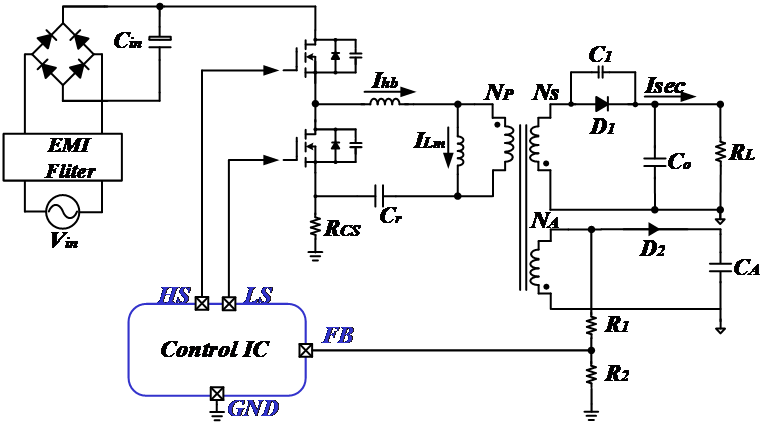
\includegraphics[width=0.8\linewidth]{figures/原边反馈电路图.png}
    \caption{原边反馈电路电路图}
    \label{fig:原边反馈电路电路图}
\end{figure}

原边反馈电路依靠辅助绕组采样输出电压,隔离变压器的特性是原边绕组、副边绕组和辅助绕组两端的电压相互成比例,原边绕组和辅助绕组电压极性相反,副边绕组和辅助绕组电压极性相同,因此辅助绕组电感电压值等于输出电压乘以副边绕组和辅助绕组的匝数比。在非对称半桥反激式开关电源系统中,在高边功率管导通阶段辅助绕组电感电压绝对值正比于原边绕组电感电压;低边功率管导通阶段辅助绕组检测副边绕组电感电压。辅助绕组电感电压VA经过R1和R2分压后得到原边反馈电压VFB送入变换器控制IC中参与闭环环路控制用以维持在负载变化情况下输出电压的稳定性。VA和VFB的电压值由式\eqref{eq:辅助绕组电压}和式\eqref{eq:VFB公式}所示:
\begin{equation}
    \label{eq:辅助绕组电压}
    V_A = \frac{N_A}{N_S}\times(V_O + V_{D1})
\end{equation}
\begin{equation}
    \label{eq:VFB公式}
    V_{FB} = V_A\times\frac{R_2}{R_1+R_2}=\frac{N_A}{N_S}\times(V_O + V_{D1})\times\frac{R_2}{R_1+R_2}
\end{equation}

\subsection{副边反馈电路}
非对称半桥反激式变换器的副边反馈电路拓扑结构如~\ref{fig:副边反馈电路电路图}所示。

\begin{figure}[htbp] 
    \centering
    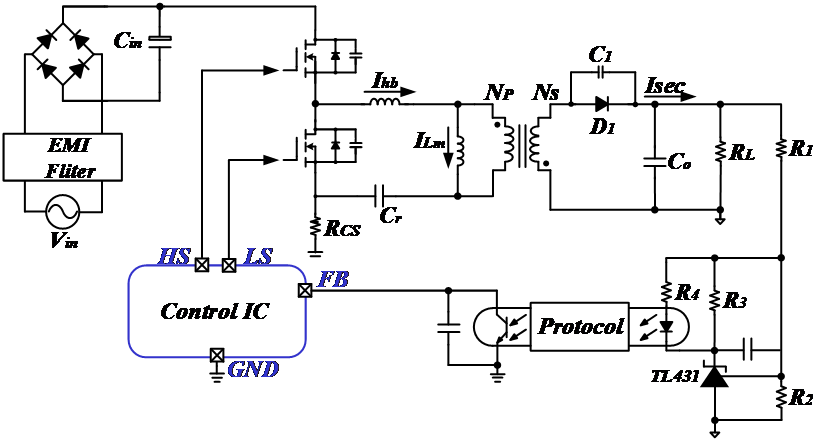
\includegraphics[width=0.8\linewidth]{figures/副边反馈电路图.png}
    \caption{副边反馈电路电路图}
    \label{fig:副边反馈电路电路图}
\end{figure}

副边反馈电路主要通过变压器副边侧基于TL431的反馈系统采集输出电压信号,该反馈系统包括输出电压分压电阻串R1和R2、TL431稳压模块、光电耦合器以及用于补偿的电容电阻。输出电压Vo通过分压电阻串R1和R2分压后送入TL431稳压模块中与其中自带的2.5V参考电压比较后产生一个误差信号,该误差信号经过光电耦合器,将电信号转化为光信号传输到变压器原边后再转化为电信号,实现变压器原副边电气隔离,TL431稳压模块可类似为一个误差放大器,通过额外的电阻电容组成的补偿网络对TL431输出的误差信号进行补偿,相当于集成在原边反馈系统变换器中的反馈网络移到了片外,可以根据不同的情况通过改变电阻电容的方式进行更精确的调节,将包含输出电压和负载电流信息的反馈电压VEA传递给变换器中。

相比于副边反馈电路,原边反馈电路由于不需要额外的外围电路,通过将反馈电压VFB输入变换器芯片内与参考电压在误差放大器中比较后输出误差放大信号Vea用于反馈环路的调节,具有较高的集成度,极大地节省了芯片外围电路板的面积,但由于副边绕组的电感电压并不完全等于输出电压,而是等于输出电压和副边续流二极管导通电压之和,导致副边绕组电感电压还可能受到负载电流和温度等因素的影响,且辅助绕组和副边绕组间存在的不匹配的情况,也将导致实际反馈电压值异于式(2-)的计算值,故而相比于副边反馈,原边反馈的采样准确性明显更低,为了消除这些误差,原边反馈电路需要添加更多的补偿电路极大增大电路设计复杂度,增大芯片的面积和功耗。因此副边反馈电路广泛应用于工业届,几乎所有的中等功率消费类电源都使用副边反馈系统。



 






















